\section{集合の圏}\label{chap-5-category-of-sets}

  圏の一例としてこれまで集合の圏を扱ってきたが、一般的な圏の射集合の定義に集合が使われていることからわかるように、集合の圏は圏論の中でも重要な役割を果たす。集合というと、集合論的な操作を想定するかもしれないが、純粋な圏論で使用するいくつかの集合の性質はたいてい圏の言葉で置き換えることができる。そのためこれから扱ういくつかの集合、とりわけ射集合を異質な存在として捉えないようにしていただきたい。

  \subsection{集合の圏と積}\label{chap-5.1-sets-and-product}
	まずは集合の圏$\cat{Set}$と積の関係性を示す。元を指定して直接直積集合を定義する方法と、普遍性を用いて直積集合の周りの写像の性質を述べて定義する方法の二つが同値であることを確認してほしい。
	\begin{define}[直積集合]\label{def-product-set}
		集合$A$と$B$の\textbf{直積集合}$A\times B$を\[A\times B =\{\tuple{a,b}\ |\ a\in A,\ b\in B\}\]と定義する。
	\end{define}
	\begin{prop}[直積と積の同値性]\label{prop-equivalence-product-set-and-product}
    $A\times B$が集合の圏$\cat{Set}$上の積$\iff A\times B$が直積集合
	\end{prop}
	\begin{proof}[$\Longrightarrow$]
		任意の元$\mor{a}{1}{A}$、$\mor{b}{1}{B}$に対して射の対の存在性により元の対$\mor{\tuple{a,b}}{1}{A\times B}$が存在する。
		また、$A\times B$の任意の元$\mor{f}{1}{A\times B}$は射影射との合成\[\pi_A\circ f=a',\ \pi_B\circ f=b'\]により、何かしらの元$a',b'$に分解できる。この時、射の対の一意性から$f=\tuple{a',b'}$が成り立つから、$f$は元の対であり順序対になる。そのため順序対とならないような元は含まれないことがわかる。

		よって実際に積$A\times B$は集合$A$と$B$の直積集合であることが示せた。
		\begin{center}
			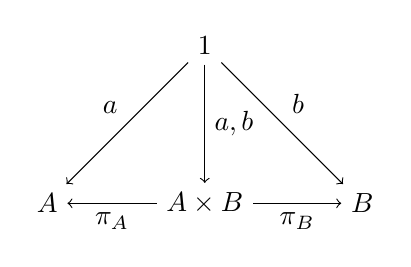
\begin{tikzpicture}[auto]
				\node (a) at (0, 0) {$A$};
				\node (b) at (4, 0) {$B$};
				\node (ab) at (2, 0) {$A\times B$};
				\node (x) at (2, 2) {$1$};
				\draw[->] (ab) to node {$\pi_A$}(a);
				\draw[->] (ab) to node[swap] {$\pi_B$}(b);
				\draw[->] (x) to node[swap] {$a$}(a);
				\draw[->] (x) to node {$b$}(b);
				\draw[->] (x) to node {$\tuple{a,b}$}(ab);
			\end{tikzpicture}
		\end{center}
	\end{proof}
	\begin{proof}[$\Longleftarrow$]
		限定的ではあるが、まずは任意の対象$X$に終対象$1$を当てはめた場合を見ていき、その後任意の対象$X$に拡張する。
		射影射となる射影写像$\pi_A,\pi_B$を任意の順序対$\tuple{a,b}$において\[\pi_A(\tuple{a,b})=a,\ \pi_B(\tuple{a,b})=b\]と定義する。

		直積集合の定義より、任意の元$a$、$b$に対して順序対$\tuple{a,b}$が存在し、順序対ではない元や重複する元を含まないことから、積の普遍性を部分的に満たすことがわかる。
		\begin{center}
			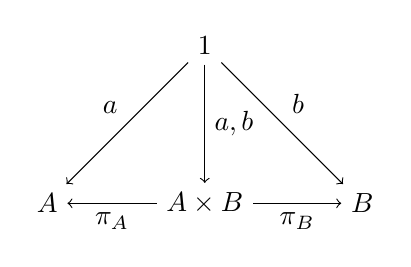
\begin{tikzpicture}[auto]
				\node (a) at (0, 0) {$A$};
				\node (b) at (4, 0) {$B$};
				\node (ab) at (2, 0) {$A\times B$};
				\node (x) at (2, 2) {$1$};
				\draw[->] (ab) to node {$\pi_A$}(a);
				\draw[->] (ab) to node[swap] {$\pi_B$}(b);
				\draw[->] (x) to node[swap] {$a$}(a);
				\draw[->] (x) to node {$b$}(b);
				\draw[->] (x) to node {$\tuple{a,b}$}(ab);
			\end{tikzpicture}
		\end{center}
		次に元の対から写像の対に拡張して考える。写像の対が一意に存在することを元の対が一意に存在することから示せばよい。

		写像$\mor{f}{X}{A}$と写像$\mor{g}{X}{B}$の写像の対$\tuple{f,g}$を$X$の任意の元$x$に対して\[\tuple{f,g}(x)=\tuple{f(x),g(x)}\]と定義する。

		また、
		\begin{align*}
			(\pi_A\circ\tuple{f,g})(x)&=\pi_A(\tuple{f,g}(x))&\text{(写像の合成の定義)}\\
			&=\pi_A(\tuple{f(x),g(x)})&\text{(写像の対の定義)}\\
			&=f(x)&\text{(元の対の可換性)}\\
			(\pi_B\circ\tuple{f,g})(x)&=\pi_B(\tuple{f,g}(x))&\text{(写像の合成の定義)}\\
			&=\pi_B(\tuple{f(x),g(x)})&\text{(写像の対の定義)}\\
			&=g(x)&\text{(元の対の可換性)}
		\end{align*}
		よって\[\pi_A\circ\tuple{f,g}=f,\ \pi_B\circ\tuple{f,g}=g\]が成り立つから写像の対は射の対としての可換性を満たすことがわかる。
		またこのような射の対は$\mor{f}{X}{A}$、$\mor{g}{X}{B}$なる任意の二射$f,g$に対し存在する。

		仮に$\pi_A\circ h=f,\ \pi_B\circ h=g$となる射$\mor{h}{X}{A\times B}$が存在しても、
		$\pi_A(h(x))=f(x),\ \pi_B(h(x))=g(x)$と元の対の一意性より$h(x)=\tuple{f(x),g(x)}$が成り立ち$h=\tuple{f,g}$となる。よって写像$f,g$の写像の対$\tuple{f,g}$は一意に存在する。
		\begin{center}
			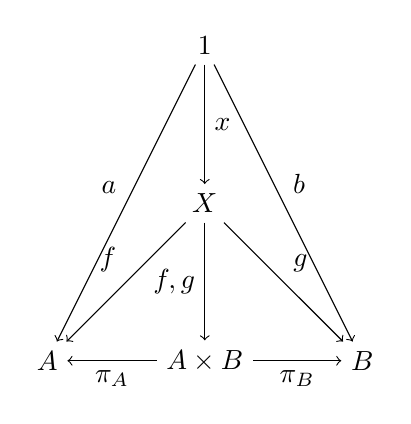
\begin{tikzpicture}[auto]
				\node (a) at (0, 0) {$A$};
				\node (b) at (4, 0) {$B$};
				\node (ab) at (2, 0) {$A\times B$};
				\node (i) at (2, 4) {$1$};
				\node (x) at (2, 2) {$X$};
				\draw[->] (ab) to node {$\pi_A$}(a);
				\draw[->] (ab) to node[swap] {$\pi_B$}(b);
				\draw[->] (x) to node[swap] {$f$}(a);
				\draw[->] (x) to node {$g$}(b);
				\draw[->] (x) to node[swap] {$\tuple{f,g}$}(ab);
				\draw[->] (i) to node[swap] {$a$}(a);
				\draw[->] (i) to node {$b$}(b);
				\draw[->] (i) to node {$x$}(x);
			\end{tikzpicture}
		\end{center}
	\end{proof}
	
  \subsection{集合の圏と終対象}
	\begin{define}[一点集合]
		何かしらの要素をただ一つ持つような集合$\{*\}$を\textbf{一点集合}とする。
	\end{define}
	\begin{prop}[一点集合と終対象の同値性]
		$1$は集合の圏$\cat{Set}$の終対象$\iff 1$は一点集合$\{*\}$
	\end{prop}
  $\cat{Set}$における終対象の一意性は、一点集合のただ一つの元を区別しないということである。
	\begin{proof}[$\Longrightarrow$]
		終対象$1$の元、すなわち射$\mor{*}{1}{1}$は終対象から終対象への射であり、恒等射ただ一つであるから終対象の元はただ一つである。
	\end{proof}
	\begin{proof}[$\Longleftarrow$]
		任意の集合$A$と一点集合$1$においてある写像$\mor{!_A}{A}{1}$が一意に存在することを示せばよい。
		任意の元$\mor{a}{1}{A}$において$!_A(a)=*$と定義すると、このような写像は任意の集合で定義できることがわかる。
		また一点集合の元がただ一つしかないので、どのような写像であっても任意の元$a$は必ず$*$に対応することになる。つまり$!_A(a)=*$以外の対応付けが行えないので写像$!_A$は一意に存在することがわかる。

		よって$A$から$1$への写像は一意に存在し、一点集合$1$は終対象となる。
	\end{proof}
	次に集合の圏に限定するが、終対象からの射を元とみなせることを証明する。

  \begin{define}[定写像]
    集合の圏$\cat{Set}$において、任意の対象$A,B$と$B$の任意の元$b$に対する\textbf{定写像}を$\mor{\varDelta b}{A}{B}$とし、$A$の任意の元$a$に対して$\varDelta b(a)=b$となる写像とする。
  \end{define}
  定写像は常に一定の値を返す定数関数のような写像である。次に元をその元を返す定写像に写す写像である、対角写像を定義する。
  \begin{define}[対角写像]
    集合の圏$\cat{Set}$において任意の対象$A,B$に対し、\textbf{対角写像}$\mor{\varDelta}{A}{\arset{Set}{B}{A}}$を$\varDelta(a)=\varDelta a$と定義する。すなわち、任意の元$a,b$に対して$\varDelta(a)(b)=a$である。
  \end{define}
	\begin{prop}[集合の元と終対象]
		任意の集合$A$とある一点集合$1$に対し$A\cong\arset{Set}{1}{A}$が成り立つ。
	\end{prop}
	\begin{proof}
    まず一点集合$1$から任意の集合$A$への射が定写像であることを示そう。\\
    これは簡単で一点集合はただ一つの元しか持たないから、それを写した先の元はただ一つに定まる。よって定写像である。\\
    対角写像$\mor{\varDelta}{A}{\arset{Set}{1}{A}}$に逆射$\mor{\varDelta^{-1}}{\arset{Set}{1}{A}}{A}$が存在することを示す。\\
    任意の射$\mor{f}{1}{A}$に対して$\varDelta^{-1}(f)=f(*)$と定義する。すると任意の射$\mor{f}{1}{A}$と任意の元$a$に対して
    \begin{align*}
      (\varDelta^{-1}\circ\varDelta)a&=\varDelta^{-1}(\varDelta a)&\text{(写像の合成の定義)}\\
      &=\varDelta a(*)&\text{($\varDelta^{-1}$の定義)}\\
      &=a&\text{(対角写像の定義)}\\
      (\varDelta\circ\varDelta^{-1})f&=(\varDelta\circ\varDelta^{-1})(\varDelta a)&\text{(fは定写像)}\\
      &=(\varDelta\circ(\varDelta^{-1}\circ\varDelta))(a)&\text{(写像の合成の定義)}\\
      &=\varDelta((\varDelta^{-1}\circ\varDelta)a)&\text{(写像の合成の定義)}\\
      &=\varDelta a&\text{(前式)}\\
      &=f
    \end{align*}
    よって\[\varDelta^{-1}\circ\varDelta=id_A,\ \varDelta\circ\varDelta^{-1}=id_\arset{Set}{1}{A}\]が成り立つから同型射であり、$A\cong\arset{Set}{1}{A}$である。
	\end{proof}

  \subsection{集合の圏と射集合}\label{chap-5.3-sets-and-arrow-sets}
	圏を定義する際に使用した射集合だが、射集合も集合であるため集合の圏の対象として捉えることができる。射集合というと、未知の集合論的な操作をいくつも持っているのかと考えてしまうが、これから扱う射集合の性質は圏論的に定義されたものだけで事足りる。そのため少し大げさかもしれないが、これから説明する操作や性質を射集合の定義だと考えても良いかもしれない。
  また、ここから一般の圏$\cat{C}$と集合の圏$\cat{Set}$を同時に扱うことになる。そのため、今扱っている対象や射、議論がどの圏上で行われるのかを意識してほしい。

  \begin{define}[共変射写像]\label{def-covariant-arrow-map}
		圏$\cat{C}$の対象$A,B$と射$\mor{f}{A}{B}$に対して、任意の射$\mor{g}{X}{A}$に射$f$を左から合成する写像を
		\begin{align*}
			&\mor{\arset{C}{X}{f}}{\arset{C}{X}{A}}{\arset{C}{X}{B}}\\
			&\arset{C}{X}{f}(g)=f\circ g
		\end{align*}
		\begin{center}
			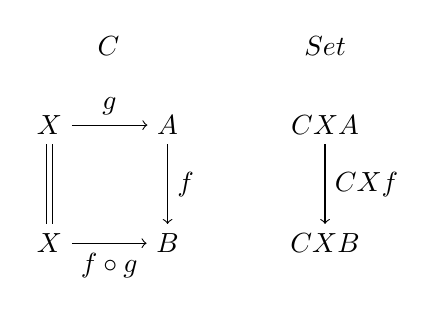
\begin{tikzpicture}[auto]
				\node (x) at (-1.5, 0) {$X$};
				\node (x2) at (-1.5, -1.5) {$X$};
				\node (a) at (0, 0) {$A$};
				\node (b) at (0, -1.5) {$B$};
				\node (ca) at (2, 0) {$\arset{C}{X}{A}$};
				\node (cb) at (2, -1.5) {$\arset{C}{X}{B}$};
				\node (catc) at (-0.75, 1) {$\cat{C}$};
				\node (catc) at (2, 1) {$\cat{Set}$};
				\draw[->] (ca) to node{$\arset{C}{X}{f}$}(cb);
				\draw[->] (a) to node{$f$}(b);
				\draw[double distance=2pt] (x) to (x2);
				\draw[->] (x) to node{$g$}(a);
				\draw[->] (x2) to node[swap]{$f\circ g$}(b);
			\end{tikzpicture}
		\end{center}
		と定義する。またこのような写像を\textbf{共変射写像}と呼ぶことにする。
	\end{define}
  
  圏の定義で確認した射の合成を行う写像\[\mor{\circ}{\arset{C}{A}{B}\times\arset{C}{X}{A}}{\arset{C}{X}{B}}\]
  は、任意の射集合の元の対$\tuple{f,g}$を$f\circ g$に写す写像であったが、共変射写像$\arset{C}{X}{f}$は対の左側の射$f$を固定した写像であることがわかる。

  また射集合の元の対$\tuple{f,g}$は積の普遍性で扱った射の対ではないことに注意してほしい。ただし、条件によっては一対一対応をすることがある。これは後で証明を行う。

  共変射写像では射を左から合成する写像を考えたが、次は射を右から合成する写像である反変射写像を考える。

	\begin{define}[反変射写像]\label{def-contravariant-arrow-map}
		圏$\cat{C}$の対象$A,B$と射$\mor{f}{A}{B}$に対して、任意の射$\mor{g}{X}{B}$に射$f$を右から合成する\textbf{反変射写像}を
		\begin{align*}
			&\mor{\arset{C}{f}{X}}{\arset{C}{B}{X}}{\arset{C}{A}{X}}\\
			&\arset{C}{f}{X}(g)=g\circ f
		\end{align*}
		\begin{center}
			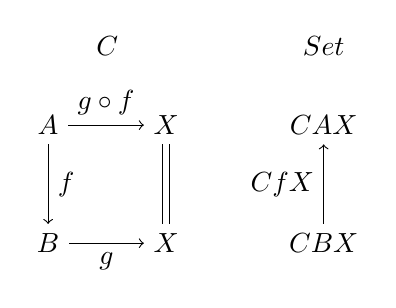
\begin{tikzpicture}[auto]
				\node (x) at (0, 0) {$X$};
				\node (x2) at (0, -1.5) {$X$};
				\node (a) at (-1.5, 0) {$A$};
				\node (b) at (-1.5, -1.5) {$B$};
				\node (ca) at (2, 0) {$\arset{C}{A}{X}$};
				\node (cb) at (2, -1.5) {$\arset{C}{B}{X}$};
				\node (catc) at (-0.75, 1) {$\cat{C}$};
				\node (catc) at (2, 1) {$\cat{Set}$};
				\draw[->] (cb) to node{$\arset{C}{f}{X}$}(ca);
				\draw[->] (a) to node{$f$}(b);
				\draw[double distance=2pt] (x) to (x2);
				\draw[->] (a) to node{$g\circ f$}(x);
				\draw[->] (b) to node[swap]{$g$}(x2);
			\end{tikzpicture}
		\end{center}
		と定義する。共変射写像と違い、射$f$に対して$\arset{C}{f}{X}$の向きが逆になっている。
	\end{define}

  これまでは一般の圏$\cat{C}$の射集合についての議論を行なってきたが、以降は射集合を取る圏を$\cat{Set}$に限定して行うことにする。理由としては$\cat{Set}$上の射集合もまた集合であり、$\cat{Set}$の対象であるためである。そのため、射集合とその始域、終域となる集合の間に射を伸ばすことができ、射集合のさらなる性質を記述することができるようになる。

  次に射写像の応用として、対象の同型との関係性を見る。

  \begin{prop}[共変射写像の同型の保存]\label{prop-covariant-arrow-map-as-isomorphism}
    ある圏$\cat{C}$において$B\cong B'\Longrightarrow$任意の対象$X$に対し$\arset{C}{X}{B}\cong\arset{C}{X}{B'}$
  \end{prop}

  \begin{proof}
    同型射を$\mor{i}{B}{B'}$、$\mor{i^{-1}}{B'}{B}$として、共変射写像\[\mor{\arset{C}{X}{i}}{\arset{C}{X}{B}}{\arset{C}{X}{B'}}\]と\[\mor{\arset{C}{X}{i^{-1}}}{\arset{C}{X}{B'}}{\arset{C}{X}{B}}\]もまた同型射になることを示す。すなわち、\[\arset{C}{X}{i}\circ\arset{C}{X}{i^{-1}}=id_{\arset{C}{X}{B'}}\]\[\arset{C}{X}{i^{-1}}\circ\arset{C}{X}{i}=id_{\arset{C}{X}{B}}\]を示せばよい。

    射集合$\arset{C}{X}{B'}$の任意の元$\mor{f}{X}{B'}$に対して、
    \begin{align*}
      \arset{C}{X}{i}\circ\arset{C}{X}{i^{-1}}(f)&=\arset{C}{X}{i}(\arset{C}{X}{i^{-1}}(f))&\text{(写像の合成の定義)}\\
      &=\arset{C}{X}{i}(i^{-1}\circ f)&\text{(共変射写像の定義)}\\
      &=i\circ i^{-1}\circ f&\text{(共変射写像の定義)}\\
      &=id_{B'}\circ f&\text{(同型射の定義)}\\
      &=f&\text{(恒等射の定義)}\\
      &=id_{\arset{C}{X}{B'}}(f)&\text{(恒等射の定義)}
    \end{align*}
    よって$\arset{C}{X}{i}\circ\arset{C}{X}{i^{-1}}=id_{\arset{C}{X}{B'}}$が示せた。同様に$\arset{C}{X}{i^{-1}}\circ\arset{C}{X}{i}=id_{\arset{C}{X}{B}}$も示せる。
    
    よって$\mor{\arset{C}{X}{i}}{\arset{C}{X}{B}}{\arset{C}{X}{B'}}$と$\mor{\arset{C}{X}{i^{-1}}}{\arset{C}{X}{B'}}{\arset{C}{X}{B}}$もまた同型射となるため、$\arset{C}{X}{B}\cong\arset{C}{X}{B'}$が成り立つ。
		\begin{center}
			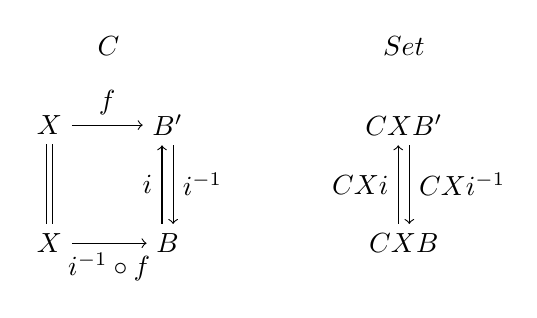
\begin{tikzpicture}[auto]
				\node (x) at (-1.5, 0) {$X$};
				\node (x2) at (-1.5, -1.5) {$X$};
				\node (a) at (0, -1.5) {$B$};
				\node (b) at (0, 0) {$B'$};
				\node (ca) at (3, -1.5) {$\arset{C}{X}{B}$};
				\node (cb) at (3, 0) {$\arset{C}{X}{B'}$};
				\node (catc) at (-0.75, 1) {$\cat{C}$};
				\node (catc) at (3, 1) {$\cat{Set}$};
				\draw[->,transform canvas={xshift=-2pt}] (ca) to node{$\arset{C}{X}{i}$}(cb);
        \draw[->,transform canvas={xshift=2pt}] (cb) to node{$\arset{C}{X}{i^{-1}}$}(ca);
				\draw[->,transform canvas={xshift=-2pt}] (a) to node{$i$}(b);
        \draw[->,transform canvas={xshift=2pt}] (b) to node{$i^{-1}$}(a);

				\draw[double distance=2pt] (x) to (x2);
				\draw[->] (x2) to node[swap]{$i^{-1}\circ f$}(a);
				\draw[->] (x) to node{$f$}(b);
			\end{tikzpicture}
		\end{center}
  \end{proof}
  
  また同様の性質が反変射写像でも成り立つ
  \begin{prop}[反変射写像の同型の保存]\label{prop-contravariant-arrow-map-as-isomorphism}
    ある圏$\cat{C}$において$A\cong A'\iff$任意の対象$X$に対し$\arset{C}{A}{X}\cong\arset{C}{A'}{X}$
  \end{prop}

  一つ前の命題の任意の対象$X$に終対象$1$を当てはめると、\[B\cong B'\Longrightarrow \arset{C}{1}{B}\cong\arset{C}{1}{B'}\]となる。$\arset{C}{1}{B}$は$B$の元の集合である。それらが同型であるということは、$B$の元と$B'$の元が一対一対応をするということであり、前に示した元と同型の関係性そのものであることが分かる。\\
  さらに任意の対象$X$に拡張することで、元$\mor{b}{1}{B}$が一対一対応をするだけでなく、射$\mor{f}{X}{B}$までもが一対一対応をすることが分かった。射の対応も元と同様に$f\sim f'$と表すことにする。

  射写像によって射集合の振る舞いを圏論的に扱えるようになった。そこで$A\cong\arset{Set}{1}{A}$によって、その間の射はどのように対応するだろうかを調べる。つまり射$\mor{f}{A}{B}$に対して$\mor{\arset{Set}{1}{f}}{\arset{Set}{1}{A}}{\arset{Set}{1}{B}}$は射$f$とどのような関係にあるか、ということである。この考えは$A$と$\arset{Set}{1}{A}$を同一視する上で有用であり、次の命題で表現できる
  \begin{prop}[元の集合の自然同型性]\label{prop-natural-isomorphism-of-element-set}
    $\arset{Set}{A}{B}\cong\arset{Set}{\arset{Set}{1}{A}}{\arset{Set}{1}{B}}$
    \begin{center}
      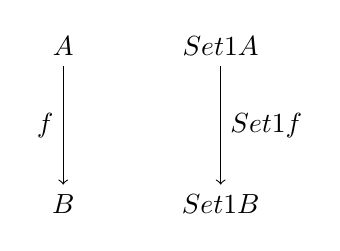
\begin{tikzpicture}[auto]
        \node (a) at (0, 2) {$A$};
        \node (b) at (0, 0) {$B$};
        \node (1a) at (2, 2) {$\arset{Set}{1}{A}$};
        \node (1b) at (2, 0) {$\arset{Set}{1}{B}$};
        \draw[->] (a) to node[swap]{$f$}(b);
        \draw[->] (1a) to node{$\arset{Set}{1}{f}$}(1b);
      \end{tikzpicture}
    \end{center}
  \end{prop}
  \begin{proof}
    \begin{align*}
      \arset{Set}{A}{B}&\cong \arset{Set}{A}{\arset{Set}{1}{B}}&\text{(共変射写像の同型の保存)}\\
      &\cong\arset{Set}{\arset{Set}{1}{A}}{\arset{Set}{1}{B}}&\text{(反変射写像の同型の保存)}\\
    \end{align*}
  \end{proof}
  またこの同型関係は図式の可換性も保つ。つまり、
  \begin{prop}[$\arset{Set}{1}{-}$の合成の保存]\label{prop-preservation-of-composition-on-1-hom-functor}
    $g\circ f = h\iff \arset{Set}{1}{g}\circ \arset{Set}{1}{f} = \arset{Set}{1}{h}$である。
  \end{prop}
  \begin{proof}[$\Longrightarrow$]
    $g\circ f=h$であるから、$\arset{Set}{1}{g}\circ \arset{Set}{1}{f} = \arset{Set}{1}{g\circ f}$を示せば良い。
    任意の射$\mor{a}{1}{A}$に対して、
    \begin{align*}
      \arset{Set}{1}{g}\circ\arset{Set}{1}{f}(a)&=\arset{Set}{1}{g}(\arset{Set}{1}{f}(a))&\text{(写像の合成の定義)}\\
      &=\arset{Set}{1}{g}(f(a))&\text{(共変射写像の定義)}\\
      &=g(f(a))&\text{(共変射写像の定義)}\\
      &=(g\circ f)(a)&\text{(写像の合成の定義)}\\
      &=\arset{Set}{1}{g\circ f}(a)&\text{(共変射写像の定義)}\\
    \end{align*}
    よって$\arset{Set}{1}{g}\circ \arset{Set}{1}{f} = \arset{Set}{1}{g\circ f}$となる。
  \end{proof}
  \begin{proof}[$\Longleftarrow$]
    $\arset{Set}{1}{g}\circ \arset{Set}{1}{f} = \arset{Set}{1}{h}$であれば、上の証明から任意の射$\mor{a}{1}{A}$に対して$\arset{Set}{1}{g}\circ \arset{Set}{1}{f}(a) =  g(f(a))$であった。また$\arset{Set}{1}{h}(a)=h(a)$も成り立つから、$g(f(a))=h(a)$であり、$g\circ f = h$となる。
  \end{proof}
  これによって元を集合の要素とみなしても、これらの同値性によって妥当であることが分かった。よって以降は紛らわしくない場合、$\mor{\varDelta a}{1}{A}$をそのまま$\mor{a}{1}{A}$と表記することにする。
  
  \begin{define}[評価射]\label{def-evaluation-arrow}
		集合の圏$\cat{Set}$の任意の対象$A,B$と$B$の元$b$、$\cat{Set}$の射$\mor{f}{B}{A}$に対して\textbf{評価射}を
		\begin{align*}
			\mor{&ev_{A,B}}{\arset{Set}{B}{A}\times B}{A}\\
			&ev_{A,B}(\tuple{f,b})=f(b)\\
		\end{align*}
		と定義する。もしくは
    これは元$b$に写像$f$を適用する操作を写像にしたものである。またこのような射は任意の対象$A,B$に対して個別に存在するが、現段階では添え字としての対象を省略し、特に区別はしない。
		厳密な証明は行わないが評価射は実際に写像になる。
	\end{define}

	\begin{define}[余評価射]\label{def-coevaluation-arrow}
		集合の圏$\cat{Set}$の任意の対象$A,B$と$A$の元$a$に対して\textbf{余評価射}を
		\begin{align*}
			\mor{&ce_{A,B}}{A}{\arset{Set}{B}{A\times B}}\\
			&ce_{A,B}(a)=\lambda x.\tuple{a,x}\mor{}{B}{A\times B}\\
			&\lambda x.\tuple{a,x}(b)=\tuple{a,b}
		\end{align*}
		と定義する。また\[ce_{A,B}(a)(b)=\tuple{a,b}\]とも表記できる。
    同様にこのような射は任意の対象$A,B$に対して個別に存在するが区別しない。
	\end{define}

  また、余評価射によって得られる射$\mor{\lambda x.\tuple{a,x}}{B}{A\times B}$と任意の射$\mor{f}{C}{B}$、$\mor{g}{A\times B}{C}$との合成に対して以下の表記を導入する。
  \begin{center}
    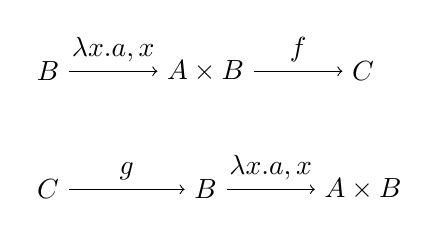
\begin{tikzpicture}[auto]
      \node (c) at (0, 0) {$C$};
      \node (b) at (2, 0) {$B$};
      \node (ab) at (4, 0) {$A\times B$};
      \draw[->] (c) to node{$g$}(b);
      \draw[->] (b) to node{$\lambda x.\tuple{a,x}$}(ab);

      \node (b) at (0, 1.5) {$B$};
      \node (ab) at (2, 1.5) {$A\times B$};
      \node (c) at (4, 1.5) {$C$};
      \draw[->] (b) to node{$\lambda x.\tuple{a,x}$}(ab);
      \draw[->] (ab) to node{$f$}(c);
    \end{tikzpicture}
  \end{center}
  \begin{align*}
    (\lambda x.\tuple{a,x})\circ f &=\lambda x.\tuple{a,f(x)}\\
    g\circ(\lambda x.\tuple{a,x}) &=\lambda x.g(\tuple{a,x})
  \end{align*}

  定義からわかるように、$B$の任意の値$b$を適用すると、
  \begin{align*}
    \lambda x.\tuple{a,f(x)}(b)&=\tuple{a,f(b)}\\
    \lambda x.g(\tuple{a,x})(b)&=g(\tuple{a,b})
  \end{align*}
  となる。
  余評価射の定義に値の適用を用いたが、これは評価射で表すことができる。次はこのような評価射と余評価射の関係性、性質を見ていく。以下証明する二つの命題は当分使用しないため、興味がなければ飛ばしてもらっても構わない。

  \begin{prop}[冪の三角恒等式1]\label{prop-triangle-identity-of-exponent-1}
    任意の対象$A,B$において、\[ce\circ \arset{Set}{B}{ev}=id_{\arset{Set}{B}{A}}\]が成り立つ。
    \begin{center}
			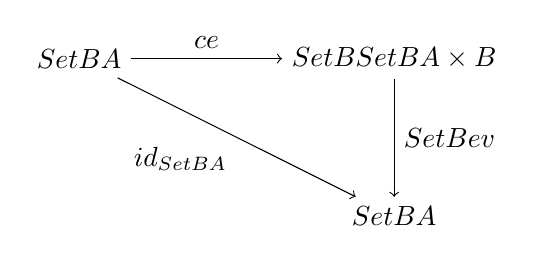
\begin{tikzpicture}[auto]
				\node (setba1) at (0, 0) {$\arset{Set}{B}{A}$};
        \node (setbbab) at (4, 0) {$\arset{Set}{B}{\arset{Set}{B}{A}\times B}$};
				\node (setba2) at (4, -2) {$\arset{Set}{B}{A}$};

				\draw[->] (setba1) to node[swap]{$id_{\arset{Set}{B}{A}}$}
        (setba2);
        \draw[->] (setba1) to node{$ce$}(setbbab);
        \draw[->] (setbbab) to node{$\arset{Set}{B}{ev}$}(setba2);
			\end{tikzpicture}
		\end{center}
  \end{prop}

  \begin{proof}
    任意の射$\mor{f}{B}{A}$に対して、
    \begin{align*}
      \arset{Set}{B}{ev}\circ ce(f)&=\arset{Set}{B}{ev}(\lambda x.\tuple{f,x})&\text{(余評価射の定義)}\\
      &=ev\circ\lambda x.\tuple{f,x}&\text{(共変射写像の定義)}\\
      &=\lambda x.ev(\tuple{f,x})\\
      &=\lambda x.f(x)&\text{(評価射の定義)}
    \end{align*}
    となる。直感的に明らかではあるが、$\lambda x.f(x)=f$を示す。
    対象$B$の任意の元$b$に対して余評価射の定義から\[(\lambda x.f(x))(b)=f(b)\]となる。よって\[\lambda x.f(x)=f\]となり、これが任意の射$f$で成り立つから、
    \[ce\circ \arset{Set}{B}{ev}=id_{\arset{Set}{B}{A}}\]となる。
  \end{proof}

  \begin{prop}[冪の三角恒等式2]\label{prop-triangle-identity-of-exponent-2}
    任意の対象$A,B$において、\[ev\circ(ce\times id_B)=id_{A\times B}\]が成り立つ。
    \begin{center}
			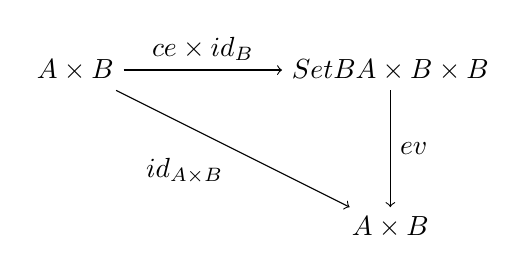
\begin{tikzpicture}[auto]
				\node (setba1) at (0, 0) {$A\times B$};
        \node (setbbab) at (4, 0) {$\arset{Set}{B}{A\times B}\times B$};
				\node (setba2) at (4, -2) {$A\times B$};

				\draw[->] (setba1) to node[swap]{$id_{A\times B}$}
        (setba2);
        \draw[->] (setba1) to node{$ce\times id_B$}(setbbab);
        \draw[->] (setbbab) to node{$ev$}(setba2);
			\end{tikzpicture}
		\end{center}
  \end{prop}

  \begin{proof}
    対象$A\times B$の任意の元$\tuple{a,b}$に対して、
    \begin{align*}
      ev\circ (ce\times id_B)(\tuple{a,b})
      &=ev(\tuple{ce(a),b})&\text{(射の積の定義)}\\
      &=ev(\tuple{\lambda x.\tuple{a,x},b})&\text{(余評価射の定義)}\\
      &=\lambda x.\tuple{a,x}(b)&\text{(評価射の定義)}\\
      &=\tuple{a,b}&\text{(余評価射の定義)}
    \end{align*}
    となる。よって\[ev\circ(ce\times id_B)=id_{A\times B}\]が成り立つ。
  \end{proof}

  \subsection{評価射、余評価射の応用}\label{chap-5.4-application-of-eval-coeval}
  評価射、余評価射を用いれば、集合の圏における圏の定義に現れる操作と等しくなるような写像を構成することができる。ここでは恒等射を得る操作と対角写像の構成を示すが、射の合成を行う操作$\mor{\circ}{\arset{Set}{B}{C}\times \arset{Set}{A}{B}}{\arset{Set}{A}{C}}$を構成することもできる。
  \begin{prop}[余評価射による恒等射の定義]\label{prop-def-identity-arrow-by-coeval}
    $\mor{\arset{Set}{A}{\pi_A}\circ ce}{1}{\arset{Set}{A}{A}}$は射集合$\arset{Set}{A}{A}$における恒等射を表す元である。

    \begin{center}
			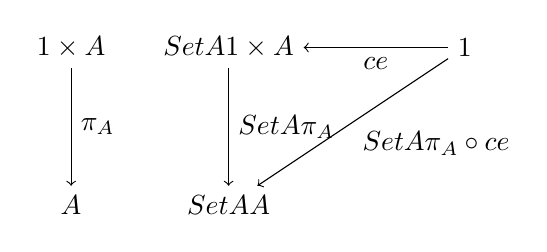
\begin{tikzpicture}[auto]
				\node (1a) at (0, 2) {$1\times A$};
        \node (a) at (0, 0) {$A$};
				\node (s1a) at (2, 2) {$\arset{Set}{A}{1\times A}$};
        \node (sa) at (2, 0) {$\arset{Set}{A}{A}$};
				\node (1) at (5, 2) {$1$};

				\draw[->] (1a) to node{$\pi_A$}(a);
        \draw[->] (s1a) to node{$\arset{Set}{A}{\pi_A}$}(sa);
        \draw[->] (1) to node{$ce$}(s1a);
        \draw[->] (1) to node{$\arset{Set}{A}{\pi_A}\circ ce$}(sa);

			\end{tikzpicture}
		\end{center}

  \end{prop}
  \begin{proof}
    $\arset{Set}{A}{\pi_A}\circ ce(*)$を計算すれば良い。\\
    \begin{align*}
      \arset{Set}{A}{\pi_A}\circ ce(*)&=\arset{Set}{A}{\pi_A}(\lambda x.\tuple{*,x})&\text{(写像の合成の定義)}\\
      &=\pi_A\circ\lambda x.\tuple{*,x}&\text{(射写像の定義)}\\
      &=\lambda x.\pi_A(\tuple{*,x})\\
      &=\lambda x.x\\
    \end{align*}
    余評価射の定義より任意の$A$の元$a$に対して$(\lambda x.x)(a)=a$であるから、$\arset{Set}{A}{\pi_A}\circ ce(*)=id_A$である。
  \end{proof}
  \begin{prop}[余評価射による対角写像の定義]\label{prop-def-diagonal-map-by-coeval}
    対角写像$\mor{\varDelta}{A}{\arset{Set}{B}{A}}$に対して、\[\varDelta=\arset{Set}{B}{\pi_A}\circ ce\]である。
    \begin{center}
			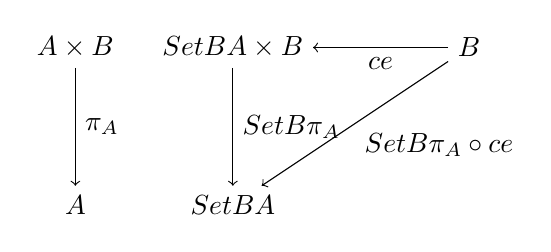
\begin{tikzpicture}[auto]
				\node (1a) at (0, 2) {$A\times B$};
        \node (a) at (0, 0) {$A$};
				\node (s1a) at (2, 2) {$\arset{Set}{B}{A\times B}$};
        \node (sa) at (2, 0) {$\arset{Set}{B}{A}$};
				\node (1) at (5, 2) {$B$};

				\draw[->] (1a) to node{$\pi_A$}(a);
        \draw[->] (s1a) to node{$\arset{Set}{B}{\pi_A}$}(sa);
        \draw[->] (1) to node{$ce$}(s1a);
        \draw[->] (1) to node{$\arset{Set}{B}{\pi_A}\circ ce$}(sa);
			\end{tikzpicture}
		\end{center}
  \end{prop}
  \begin{proof}
    $A$の任意の元$a$に対して、
    \begin{align*}
      \arset{Set}{B}{\pi_A}\circ ce(a)&=\arset{Set}{B}{\pi_A}(\lambda x.\tuple{a,x})&\text{(写像の合成の定義)}\\
      &=\pi_A\circ\lambda x.\tuple{a,x}&\text{(射写像の定義)}\\
      &=\lambda x.\pi_A(\tuple{a,x})\\
      &=\lambda x.a
    \end{align*}
    恒等射と同様に、$B$の任意の元$b$に対して$\mor{\lambda x.a}{B}{A}$は$(\lambda x.a)b=a$を満たす。よって$\lambda x.a$は定写像であり、$\lambda x.a=\varDelta (a)$である。\\
    $\arset{Set}{B}{\pi_A}\circ ce(a)=\varDelta (a)$が成り立つから、$\varDelta=\arset{Set}{B}{\pi_A}\circ ce$である。
  \end{proof}